\subsection{The NEPOMUK Social Semantic Desktop}
\label{sub:nepomuk}

We have seen so far a multitude of systems which use semantic technologies to enable better management of personal information. We continue by describing the NEPOMUK Semantic Desktop in more detail, as it is the framework we chose for the research presented in this thesis. In the section to follow, we sum up the systems in an analysis and a discussion of their characteristics.

Build on the ideas described in \cite{Decker2004}, the NEPOMUK project aims to bring together Semantic Web technologies applied on the desktop for better PIM, along with Peer-to-Peer technology and social networks for better collaboration and sharing of information.

NEPOMUK started as an EU research project, involving partners from academia and industry. It set out to define the blueprint \cite{Bernardi2008} for a generic Semantic Desktop, based on previous research as well as new studies. Many of the systems presented above were surveyed, and many of the pioneers of the Semantic Desktop research were involved. The partners contributed knowledge and existing useful components. 

The report on the NEPOMUK final architecture \cite{Reif2008} describes how the Semantic Web technologies are applied on local scale --- ``to integrate information between applications such as email, contacts, calendars, or file-manager'', and on the global scale --- ``users socially interact by sharing resources, by communicating, and by collaborating over the network''. 
The resulting Semantic Desktop brings improvements in two distinct but intertwined directions: enhanced Personal Information Management through better interlinking of information across application boundaries, as well as improved information sharing and exchange across social and organisational boundaries.

\subsubsection{The Blueprint of a Semantic Desktop}

The main goal of NEPOMUK was to define a well-thought blueprint for the Semantic Desktop, which was to provide a template for frameworks to follow, and generic solutions to the design problems which arose. The blueprint evolved based on requirements and the final version is described in \cite{Reif2008}.
It was continuously used to provide a prototype reference implementation of the framework. There were also prototypes for special community scenarios, and usage studies done on them, which fed back into the blueprint design.

The blueprint of the Social Semantic Desktop as envisioned by NEPOMUK is defined on two dimensions:
\begin{enumerate}
 \item the way the mental model of the user is represented by the framework, and
 \item the services provided by the system to the users.
\end{enumerate}

The first item in the list --- the representation of the mental model --- is described in more detail in the specification, as it is a crucial point enabling communication and data sharing across any future Semantic Desktop which follows the blueprint. For the second item, the blueprint does not provide recommendations on the exact architecture of the system, leaving this issue to the implementers to decide. General guidelines are given on the basic services required, like the storage service for example.

\subsubsection{Describing the Mental Model --- the NEPOMUK Ontologies}

The NEPOMUK Semantic Desktop defines and uses a set of ontologies\footnote{\url{http://oscaf.sourceforge.net/}, previously found at \url{http://www.semanticdesktop.org/ontologies/}}, known as ``the NEPOMUK ontologies'', or ``the desktop ontologies'', which are complemented by ontologies defined by the community, like Xesam\footnote{\url{http://xesam.org/main/XesamOntology} - is used in Nepomuk-KDE}. 
They describe as completely as possible the way knowledge representation is done in the system, from the very high level concepts to the most detailed low level ones. Figure \ref{fig:ontologiespyramid} \cite{Reif2008} shows how the ontologies build and depend on each other. The pyramid is divided into three levels, the top two levels containing ontologies which are more stable, and provided as part of the framework, while the bottom layer ontologies are customisable by users. 

\begin{figure}[tb]
 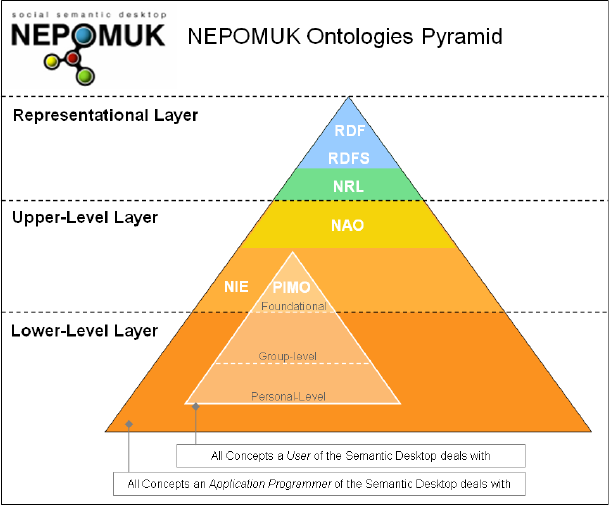
\includegraphics[width=0.8\linewidth]{chapters/background/img/ontologies.png}
\caption{The pyramid of desktop ontologies.}
\label{fig:ontologiespyramid}
\end{figure} 

To accommodate some restrictions specific to describing desktop and personal data, an extension to RDF was developed. It is called NEPOMUK Representational Language (NRL)\footnote{\url{http://oscaf.sourceforge.net/nrl.html}, previously at \url{http://www.semanticdesktop.org/ontologies/nrl}} \cite{Sintek2007}, and is a representational ontology, thus belonging in the top level of the pyramid. It adds Named Graphs and Graph Views to RDF/S and introduces the closed world assumption to the data. The named graphs in NRL are similar to the named graphs defined by \cite{Carroll2005} except that they do not follow the open world assumption. NRL defines graph roles for named graphs, where roles contain information about a graph's data and how it should be handled.

The open world assumption which is usually used on the Web, states that everything that is not known is undefined, which makes sense when working with very large amounts of information, most of it unknown. It does not work as well on the desktop, where we handle personal data that is implicitly known to the user in its entirety. That is why NRL introduces the closed world assumption, which states that everything that is unknown is false. However, NRL does not make any assumptions on the semantics of a graph defined with it. With the use of graph views over named graphs, there can possibly exist different views with different semantics over the same graph.

The upper level ontologies describe basic concepts generalising over multiple domains and activities specific to the desktop and PIM. There are three ontologies in this level: 
\begin{description}
 \item[NEPOMUK Annotation Ontology] (NAO\footnote{\url{http://oscaf.sourceforge.net/nao.html}, previously at \url{http://www.semanticdesktop.org/ontologies/nao/}}) contains concepts which allow users to annotate desktop resources, including custom descriptions, identifiers, tags and ratings. Generic relationships between related resources can be made explicit through properties defined in this ontology.
 \item[NEPOMUK Information Element Ontology] (NIE\footnote{\url{http://oscaf.sourceforge.net/nie.html}, previously at \url{http://www.semanticdesktop.org/ontologies/nie/}}) describes a unified vocabulary for native resources available on the desktop. NIE is in fact a larger framework, where the core part is the NIE ontology, complemented by several smaller vocabularies describing specific types of desktop resources, like files, music, emails, address book contacts, calendar entries, etc. Standards for representating many of these types already existed, either in the form of RFCs or in the form of Web vocabularies. In these cases, the existing resources were used as basis for the respective NEPOMUK ontologies. For example, the NEPOMUK Contact Ontology (NCO\footnote{\url{http://oscaf.sourceforge.net/nco.html}, previously at \url{http://www.semanticdesktop.org/ontologies/nco/}}) was designed based on the VCARD specification (RFC 2426 \cite{RFC2426}), and on the Vcard ontology\footnote{\url{http://www.w3.org/TR/
vcard-rdf/}}, but it has a much broader scope than either of the two. Similarly, the NEPOMUK Calendar Ontology (NCAL\footnote{\url{http://oscaf.sourceforge.net/ncal.html}, previously at \url{http://www.semanticdesktop.org/ontologies/ncal/}}) is an extended adaptation of the W3C calendaring ontology\footnote{\url{http://www.w3.org/2002/12/cal/}}. NIE defines two disjunct classes of resources, \verb|DataObject|s --- the physical representation, and \verb|InformationElement|s --- the interpretation and content of resources. The two are then subclassed in each specific vocabulary of the framework. The NIE classes are designed for machine use in extracting semantic information from existing desktop sources and applications, not for direct handling by the users.
 \item[Personal Information Model Ontology] (PIMO\footnote{\url{http://oscaf.sourceforge.net/pimo.html}, previously at \url{http://www.semanticdesktop.org/ontologies/pimo/}}) is both a upper level ontology and a lower level ontology, as it contains both generic concepts and quite specific ones. From a user's point of view, PIMO is the central ontology of the Semantic Desktop. Its scope is to model the data that the user works with. According to its specification \cite{Sauermann2009a}, ``PIMO is based on the idea that users have a mental model to categorize their environment'', and ``each concept in the environment \dots is represented as [a] Thing in the model''. PIMO defines high level types like Person, Project, Event and Task, which reflect the user's mental image of the objects, not their representation in various desktop applications, nor the files used to store the information about them. That is the task of the NIE ontology and framework, while the PIMO is needed to provide an aggregated view of all 
the possible sources of information about a \emph{thing} the user needs.
\end{description}

The lower level ontologies consist of domain ontologies and application ontologies --- which have very specific or limited use cases. 
Users can import new ontologies into their Semantic Desktop either directly or through applications. When certain ontologies become widely used, it is recommended that they go through a process of standardisation and are included in the desktop ontologies, in order to support reuse. 

Existing ontologies can be customised by users or by application developers, this is however discouraged for the upper level ontologies, as it would affect interoperability between Semantic Desktops.

\subsubsection{The NEPOMUK Reference Implementation}

The reference implementation of NEPOMUK is based on the blueprint defined within the project, but it is not an exact realisation of it. The general structure is maintained however, and several of the possible services are provided. The implementation is done in Java, for portability.

\begin{figure}[tb]
 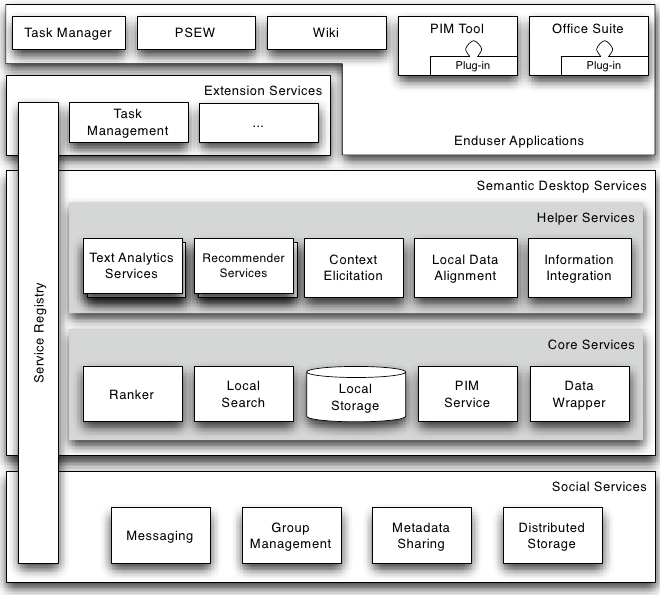
\includegraphics[width=0.8\linewidth]{chapters/background/img/javaarchitecture.png}
\caption{The architecture of the NEPOMUK Java implementation.}
\label{fig:nepomukjava}
\end{figure} 

The service oriented architecture of the Java implementation of NEPOMUK uses SOAP and OSGi for communications between the services, and for discovery. The component which provides the registry and discovery functionality is called the NepomukMiddleware (or Middleware), and it is a service itself. The implementation evolved from a local web server with SOAP, to Eclipse, as it has better support for inter-service communication.

Figure \ref{fig:nepomukjava} \cite{Reif2008} shows the services composing the reference implementation. The core services provide functionalities for extraction, storage, and retrieval of the semantic desktop data. They are fundamental for the functionality of the Semantic Desktop, as they are used by all the other helper services and applications built on top of the framework. 

The storage service is the central service of the Semantic Desktop. All the semantic data is stored and retrieved from here, thus acting as a blackboard (see Section \ref{sub:characteristicsofsd}). The storage service uses existing triple store implementations, current version using Sesame2. Additionally it provides some basic inference and query support. Lucene is used for indexing. 

The DataWrapper service extracts information from desktop sources and stores it in semantic form in the central RDF store. It uses plugins to access and extract data from application specific formats and repositories. Other helper services can be combined with the DataWrapper, to ensure that the data is well integrated and that duplicates are removed (e.g. an integration service), a data alignment service, or an inference service to extract new information based on the existing triples. 

The PIM service provides convenience methods to access and create information in a user's PIMO. 

The local search service provides search functionality over the local repository, supporting both structured queries and full text search. It includes the functionality provided by a Ranker service, which computes resource relevance for better search results. 

Additional helper services were developed: a Context service, Recommender services, Text Analytics services. 
On top of the core services and the helper services, several extension services were developed, to showcase possible uses and to demonstrate how the services can be combined. 
On top of the services, applications were built to provide functionality to the users in a friendly user interface. The interface to this implementation of the NEPOMUK Semantic Desktop is called PSEW (Personal Knowledge Workbench) \cite{Grimnes2009}. It offers a visual way of interacting with the services, as well as several views of the data contained in the local repository. Other specialised applications were developed: a semantic email extension \cite{Scerri2009} to Microsoft Outlook and to Mozilla Thunderbird, a plugin for Microsoft Word \cite{Groza2011} to semantically annotate documents, etc.

The social part of the Social Semantic Desktop was meant to be fully distributed, thus a P2P network implementation was used for the majority of the services. However, a centralised NepomukHub was developed as well, using XMPP. The NepomukHub acts as a server for inter [Semantic] Desktop communication, passing messages between NEPOMUK instances, and also as a shared triple store, where social information, like group memberships, is stored and managed. The messages sent through the NepomukHub transport RDF graphs, thus any semantic information can be shared among desktops. Several social services were developed on top of the P2P network and the NepomukHub infrastructure. They include a Messaging service, a Metadata Sharing service, a Distributed Storage service and Distributed Search. Local services can be extended to use the social services.

\subsubsection{Nepomuk-KDE}

By far the most successful part of the NEPOMUK project was the ``Mandriva Community scenario'' \cite{Lauriere2006} or Nepomuk-KDE\footnote{\url{http://nepomuk.kde.org}} as it became known. It was initially meant as a proof of concept, showing that the blueprint can be realised outside of the reference implementation. The start of the NEPOMUK project coincided roughly with the beginning of development on a new major version of the KDE\footnote{KDE has been rebranded in the mean time to refer to the community instead of the software produced. Thus KDE is no longer an acronym for ``K Desktop Environment''.} Desktop Environment for Linux --- KDE4. Thus it provided the opportunity of including the new research ideas into an emerging platform, more deeply than it could have been done for a system that was already completely designed and implemented. As a result, Nepomuk-KDE is part of the core libraries of KDE and is used in several central applications, the best example being Dolphin, the default file manager. 
Desktop search is also done through NEPOMUK, and metadata creation, such as tagging, rating and commenting, is available desktop-wide. The adoption of NEPOMUK and semantic technologies has been very good, and development on the framework continued after the end of the EU project, driven by the community that was formed.

Including NEPOMUK in KDE also meant convincing the developers of KDE applications to make their software use the new semantic features. It required familiarising them with the semantic technologies used, and encouraging them to participate in the development of the framework and to collaborate on the ontologies. 

For open source projects like KDE, there are restrictions on what libraries can be reused due to software licences. This had an effect in the first stages, on the fact that the Java code of the NEPOMUK reference implementation could not be directly reused. Although it is possible to run Java on Linux, there are restrictions on the distribution of Java libraries. That was one of the reasons why Qt, the language in which KDE is developed, was preferred for Nepomuk-KDE. Although it is possible to use Java libraries in applications, code written in Qt/C++ was preferred by the packagers of the distributions that used KDE4. Thus, despite inferior results and features, many Nepomuk-KDE Semantic Desktops used the Redland\footnote{\url{http://librdf.org/}} C library for the storage service, while at the same time Sesame2 library was available but since it was written in Java, it required additional configuration. Currently Nepomuk-KDE uses a customised trimmed down version of OpenLink's Virtuoso\footnote{\url{http://
virtuoso.openlinksw.com/}}. It is feature-rich, stable, and the close collaboration with the OpenLink developers resulted in a version tailored specifically for running a triple store on a desktop.

Architecture-wise Nepomuk-KDE differs from the blueprint. For simplicity the social part has been ignored in the start, and the focus was on providing easy and simple to use semantic features to attract more contributors before diving into more complex tasks. Several social aspects are being implemented now with the use of NEPOMUK in the Telepathy\footnote{\url{http://telepathy.freedesktop.org/}} project.

The services in Nepomuk-KDE are also different. The preferred inter-service communication method is either through DBus\footnote{\url{http://www.freedesktop.org/wiki/Software/dbus}} or API calls. The services themselves are not defined as Web services running on the desktop, but as KDE modules. They are managed through a NepomukServer service.
As already mentioned, the current implementation of the Storage service uses Virtuoso as the default triple store, although other backends can be configured for use. 
The Data Wrapper function is done by Strigi\footnote{\url{http://strigi.sourceforge.net/}}, but instead of independent plugins for external applications, Strigi is a plugin-based system, with each plugin being responsible for certain types of files. Other exporters of semantic data come from Akonadi\footnote{\url{http://community.kde.org/KDE_PIM/Akonadi}}, the PIM framework of KDE.

The Nepomuk-KDE framework is changing continuously, due to the active community around it. It is evolving together with KDE and because of it, the uptake has been considerable, with many developers adding semantic features to their applications, and thus increasing the visibility and attracting more users.
